\documentclass[12pt]{article}

\usepackage[utf8]{inputenc}%encodage des caractères
\usepackage[T1]{fontenc}%encodage de la police
\usepackage[french]{babel}%langue française
\usepackage{hyperref}
\usepackage{amsmath}
\usepackage{graphicx}
\usepackage{xcolor}
\usepackage{amsmath}

\title{Jeu de Hex}
\author{}
\date{\today}

\begin{document}

\maketitle
\thispagestyle{empty}
\setcounter{page}{0}

\newpage
\tableofcontents
\newpage

\section{Introduction}

	\subsection{Présentation : jeu de hex}
	
Le jeu d'hex est un jeu très simple qui se joue à deux joueurs, l'un contre l'autre. Le plateau du jeu se présente sous la forme d'une grille d'hexagones. Le but des deux joueurs est de remplir les cases tour par tour de leur couleur. La partie se termine quand l'un des joueurs à relié deux côtés opposés avec sa couleur.

\begin{figure}[ht]
  \begin{center}
    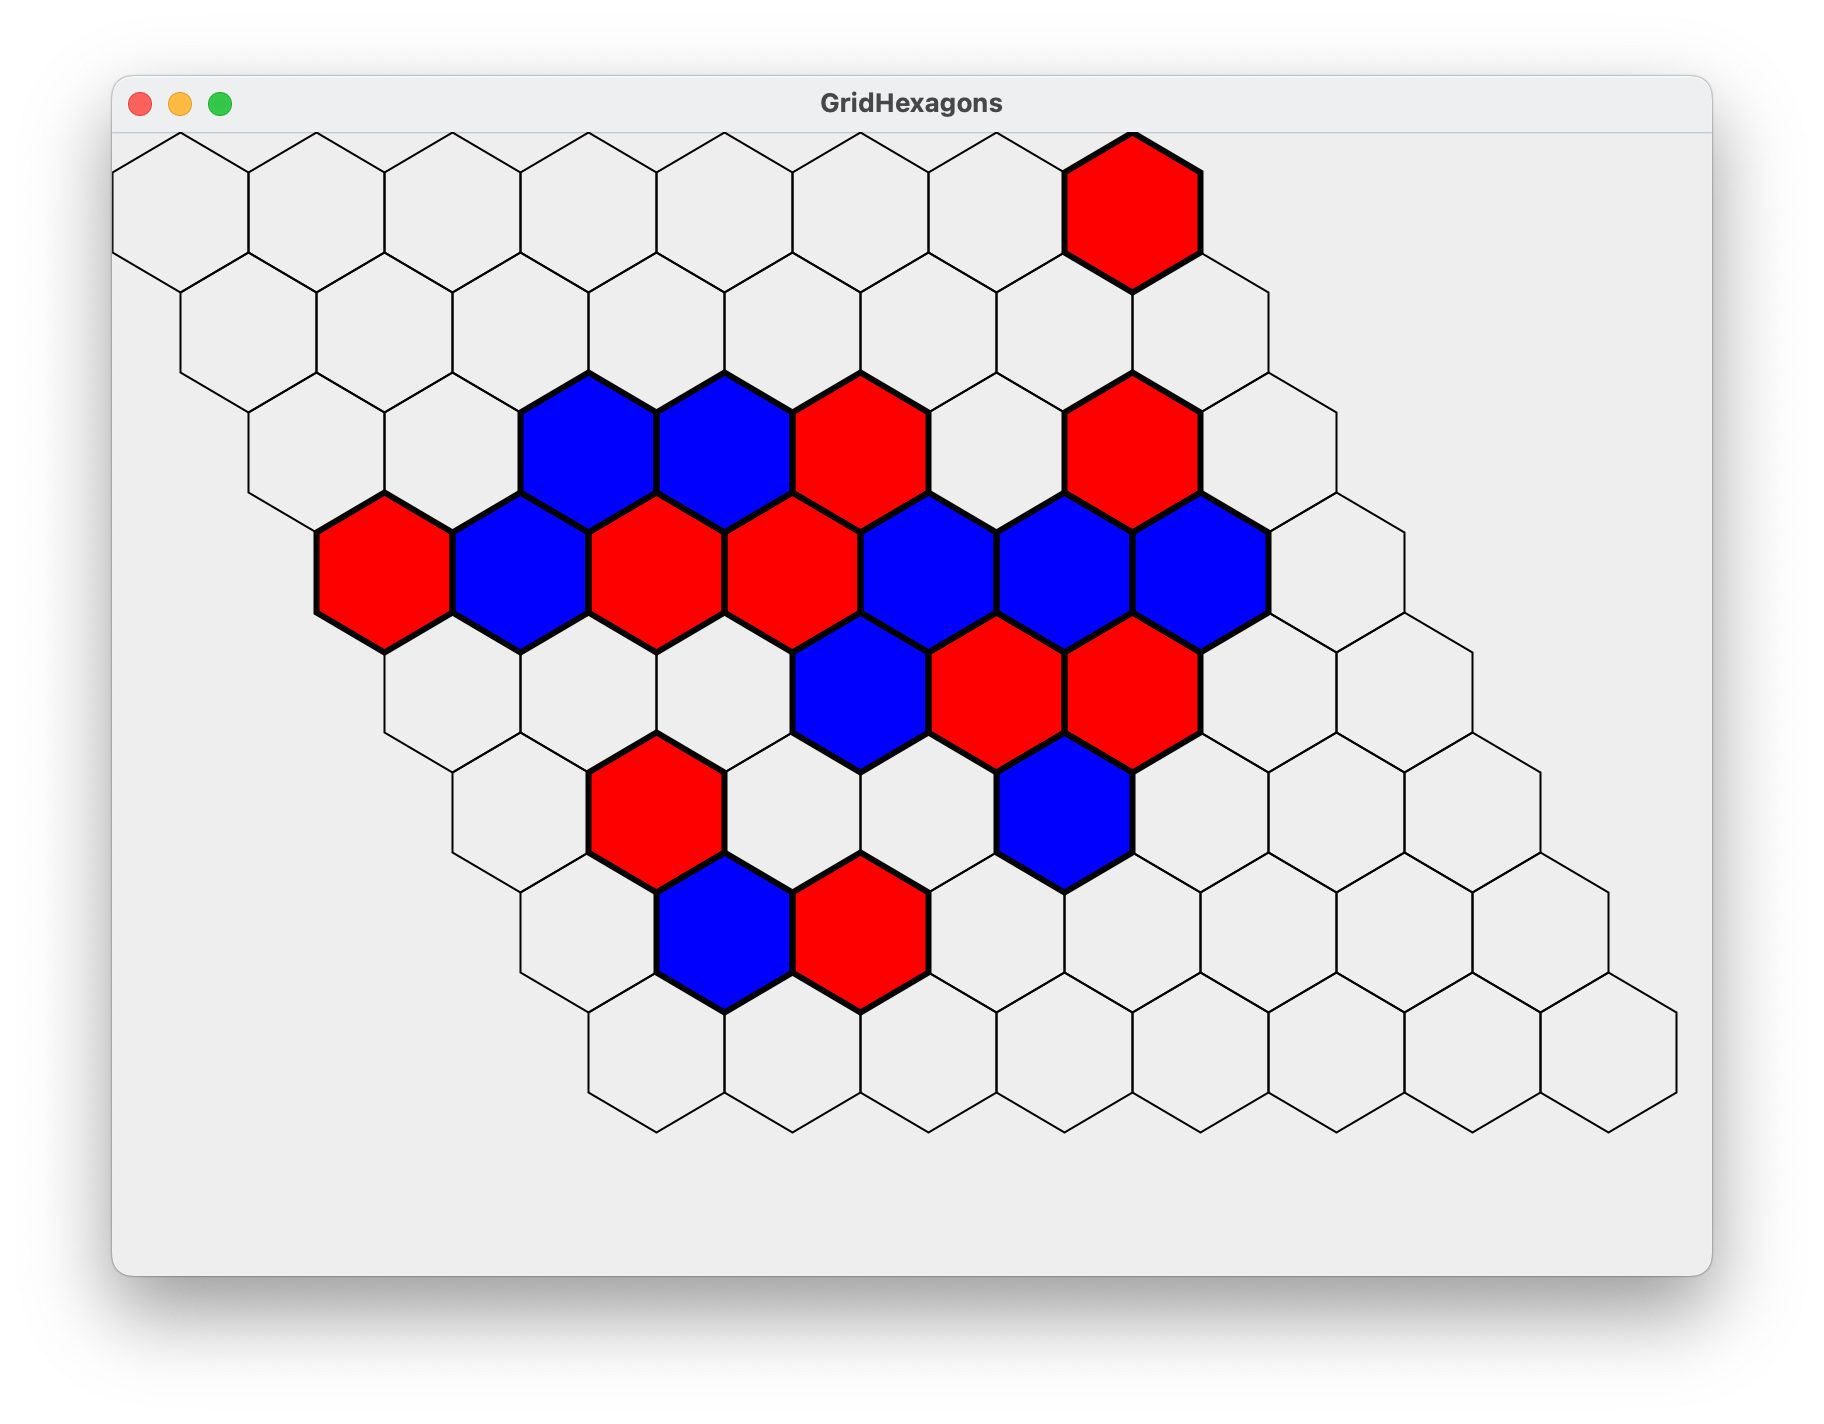
\includegraphics[width=1\textwidth]{./images/Board} 
  \end{center}
  \caption{Plateau de jeu}
\end{figure}

	\subsection{Plan Rapport}

\section{Objectif}

	\subsection{Grandes étapes}
	
\begin{enumerate}
	\item Implémenter le jeu de hex
	\begin{itemize}
		\item les règles du jeu
		\item l'interface graphique du jeu
	\end{itemize}
	\item Implémenter l'algorithme de recherche Monte Carlo ( MCTS ) 
	\item Faire des test avec l'algorithme de recherche MCTS 
\end{enumerate}

	\subsection{Problèmatique}

Le jeu de hex est un jeu où l'on est face à un adversaire, le but est de terminer premier à traverser le plateau. On peut donc supposer qu'il existe des stratégies pour remporter plus facilement les parties du jeu de hex. Pour savoir si on peut vraiment avoir un avantage sur notre adversaire on va utiliser l'algorithme MCTS. l'algorithme MCTS fonctionne avec un system de budget qui correspond au nombre de simulation que l'algorithme va faire pour déterminer le meilleur coup. La taille du plateau a aussi son importance car elle augmente le nombre de possibilités de jeu.


\textbf{Ce qu'on cherche donc à savoir est si on varie le budget des joueurs et la taille du plateau cela influe sur le résultat final du jeu ?}

	\subsection{Historique Monte Carlo}
	
La méthode de Monte-Carlo à vue le jour la première fois en 1993, écrite par Bernd Brügmann mais l'idée de l'algorithme n'a pas vraiment était pris au sérieux au début. En 2000 les chercheurs Bruno Bouzy, Tristan Cazenave et Bernard Helmstetter améliore l'idée de Bernd Brügmann mais sans que cela vienne surpasser les programmes actuels.


Il faut attendre 2006 avant que le programme Crazy Stone, utilisant l'algorithme de recherche Monte-Carlo ne dépasse les autres programmes de recherche sur jeu de go avec un plateau 9x9. En 2007 le programme MoGo va surpasser tous les autres programme en finissant premier lors de la Computer Olympiad sur un plateau 19x19.


Les programmes Crazy Stone et MoGo vont continuer de s'améliorer jusqu'à battre des joueurs professionnels en 2008. Mais les deux programmes restent à ce jour plus faibles que les meilleurs joueurs de go.


\section{Algorithme}

	\subsection{algorithme de recherche Monte Carlo}
	
		\subsubsection{Description}
		
\section{Sources}

https://interstices.info/le-jeu-de-go-et-la-revolution-de-monte-carlo/

		



\end{document}
